\documentclass[a4paper,12pt]{memoir}
\usepackage{fontspec}
\usepackage{courier}
\usepackage{polyglossia}
\usepackage{hyperref}
\usepackage{graphicx}
\usepackage{listings}
\usepackage{xcolor}
\usepackage{listings}
\usepackage{egyptian}
\lstset{basicstyle=\ttfamily\footnotesize,language=Python,backgroundcolor = \color{lightgray},showstringspaces=false,columns=fullflexible,showstringspaces=false, morestring=[b]", morestring=[b]',keepspaces=true,
escapeinside={(*@}{@*)}}
\newtheorem{theorem}{Theorem}[section]
\newtheorem{exercise}[theorem]{Άσκηση}
\setmainlanguage{greek}
\setromanfont{Candara}
\setsansfont{Calibri}
\setmonofont{Consolas}

\newcommand{\sel}[1] {(Στο βιβλίο βρίσκεται στη Σελ. #1)}
\begin{document}
\title{$A\lambda\gamma\epsilon\beta\rho y$ \\ Μαθηματικά Γυμνασίου με Python}

\author{Δημήτρης Νικολός}
\maketitle
\chapter{Τι θα χρησιμοποιήσουμε;}
\section{Η γλώσσα προγραμματισμού Python}
Σε αυτές τις σημειώσεις θα χρησιμοποιήσουμε τη γλώσσα προγραμματισμού Python και μάλιστα την έκδοση 3. Υπάρχει και Python 2 αλλά υπάρχουν σχέδια για την αντικατάστασή της από την Python 3. Για να εγκαταστήσεις την Python 3 θα πρέπει να την κατεβάσεις από το επίσημο site της Python \href{https://www.python.org/}{www.python.org}. Κατεβάστε την πιο πρόσφατη έκδοση που σας προτείνει θα είναι κάτι σαν 3.8.2 ή κάτι 

\section{Ο επεξεργαστής προγραμμάτων Mu}
Μπορείς να γράψεις Python σε οποιοδήποτε πρόγραμμα υποστηρίζει απλό κείμενο, ακόμη και στο Σημειωματάριο, όμως σε αυτές τις σημειώσεις χρησιμοποιούμε τον επεξεργαστή Python, Mu Editor ή πιο απλά Mu που μπορείς να τον κατεβάσεις από τη σελίδα \href{https://codewith.mu/}{codewith.mu}. Μόλις το ανοίξεις θα δεις την εικόνα \ref{Mu}. 
\begin{figure}
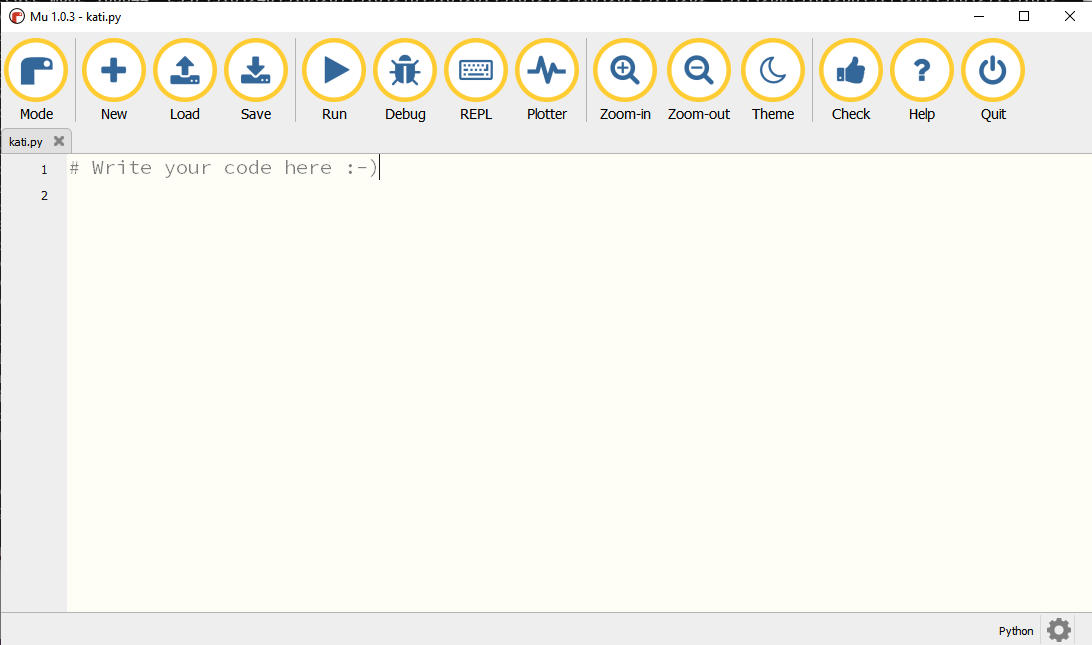
\includegraphics[width=\textwidth]{mu.png}
\label{Mu}
\caption{Mu: Ένας επεξεργαστής προγραμμάτων Python}
\end{figure}

Μπορείς να πατήσεις την εκτέλεση (κουμπί Run) και τότε θα δεις ότι το παράθυρο χωρίζεται σε δύο τμήματα (Εικόνα \ref{Mu2}).  Αν θες να δοκιμάσεις ένα ολόκληρο πρόγραμμα μπορείς να το πληκτρολογήσεις στο βασικό παράθυρο (τώρα γράφει `\#Write your code here`). Ενώ αν θες να δοκιμάσεις κάποια εντολή τότε μπορείς να την πληκτρολογήσεις στο κάτω παράθυρο (τώρα γράφει $>>>$).  Το κάτω παράθυρο ονομάζεται REPL, από τα αρχικά των λέξεων Read, Eval, Print, Loop δηλαδή Διάβασε, Εκτέλεσε (την εντολή/έκφραση), Τύπωσε, Επανάλαβε. Το REPL θα διαβάσει την εντολή, θα την εκτελέσει και θα μας δώσει το αποτέλεσμα.

Από εδώ και πέρα όταν βλέπετε στις σημειώσεις τα τρία σύμβολα ``μεγαλύτερο από'' ($>>>$) θα πληκτρολογείτε τις αντίστοιχες εντολές στο κάτω παράθυρο (REPL). Τα μεγαλύτερα προγράμματα που δεν θα έχουν αυτό το σύμβολο θα τα πληκτρολογείτε στο πάνω παράθυρο.

\fbox{
	\parbox{0.8\textwidth}{%
	\textbf{Συμβουλή:} Αν χρησιμοποιείτε την ηλεκτρονική έκδοση αυτών των σημειώσεων, θυμηθείτε να πληκτρολογείτε τις εντολές και να μην τις κάνετε αντιγραφή επικόλληση.
	}
}


Στην αρχή θα δοκιμάσεις κάποια πράγματα στο κάτω παράθυρο, όμως μην ανησυχείς σύντομα θα γράφεις τα δικά σου προγράμματα στο πάνω παράθυρο.

\begin{figure}
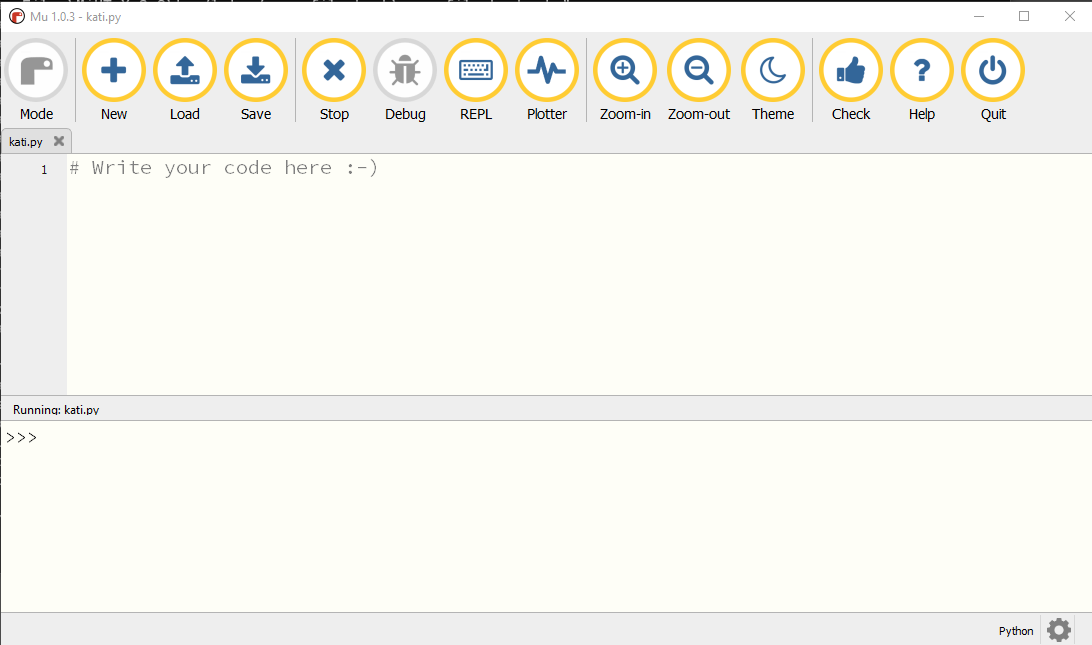
\includegraphics[width=\textwidth]{mu2.png}
\label{Mu2}
\caption{Το πρόγραμμα Mu όταν εκτελείτε ένας κώδικας}
\end{figure}

\section{Το βιβλίο μαθηματικών της Α΄ Γυμνασίου}
Σε αυτές τις σημειώσεις οι περισσότερες ασκήσεις είναι από το βιβλίο Μαθηματικών της Α΄ Γυμνασίου των Βανδουλάκη, Καλλιγά, Μαρκάκη και Φερεντίνου (Εικόνα \ref{matha}).

\begin{figure}
\centering
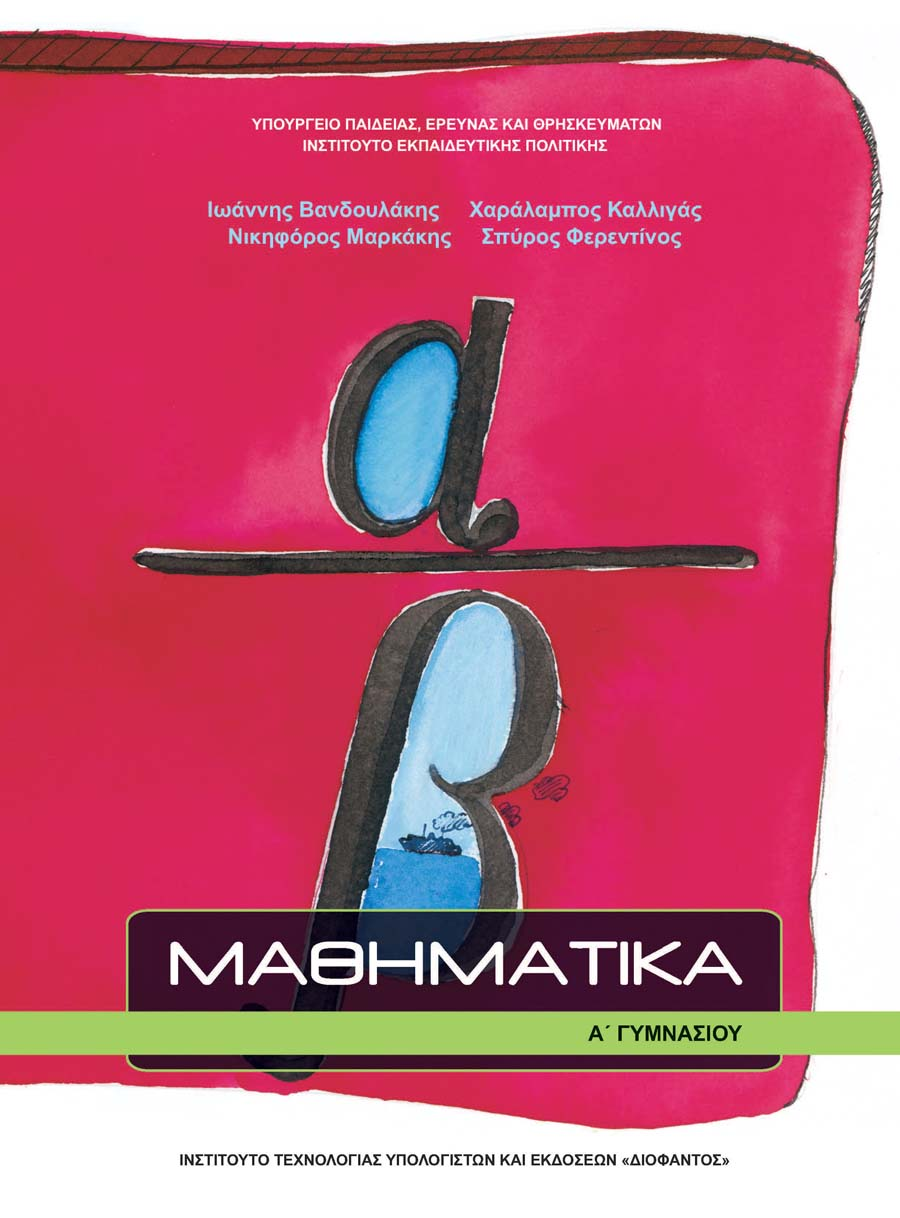
\includegraphics[width=0.8\textwidth]{matha.jpg}
\label{matha}
\caption{Το εξώφυλλο του βιβλίου των Μαθηματικών που θα χρησιμοποιήσουμε}
\end{figure}
\chapter{Φυσικοί αριθμοί}

\section{Οι αριθμοί και η Python}

Οι φυσικοί αριθμοί είναι οι αριθμοί από 0, 1, 2, 3, 4, 5, 6, \ldots, 98, 99, 100, \ldots, 1999, 2000, 2001, \ldots

Η Python μπορεί να χειριστεί φυσικούς αριθμούς. Δοκιμάστε να γράψετε στο REPL έναν φυσικό αριθμό, θα δείτε ότι η Python θα τον επαναλάβει. Π.χ. δείτε τον αριθμό εκατόν είκοσι τρια (123).
\begin{lstlisting}
>>> 123
123
\end{lstlisting}

Στην Python όμως θα πρέπει να ακολουθείς κάποιους επιπλέον κανόνες. Για παράδειγμα στους αριθμούς δεν πρέπει να βάζεις τελείες στις χιλιάδες όπως στο χαρτί. Αν το κάνεις στην καλύτερη περίπτωση θα προκύψει κάποιο λάθος, στην χειρότερη ο υπολογιστής θα καταλάβει διαφορετικό αριθμό από αυτόν που εννοείς.
Δείτε το παρακάτω παράδειγμα στο REPL.
\begin{lstlisting}
>>> 1.000.000
  File "<stdin>", line 1
    1.000.000
            ^
SyntaxError: invalid syntax
>>> 100.000
100.0
\end{lstlisting}
Σε αυτό το παράδειγμα, η Python δεν καταλαβαίνει καθόλου τον αριθμό 1.000.000 γραμμένο με τελείες ενώ μεταφράζει το 100.000 σε 100.0, που για την Python σημαίνει 100 (εκατό). Γι' αυτόν τον λόγο δεν βάζουμε καθόλου τελείες έτσι αν θέλουμε να γράψουμε το ένα εκατομμύριο θα γράψουμε 1000000.
\begin{lstlisting}
>>> 1000000
1000000
\end{lstlisting}

\section{Πρόσθεση, αφαίρεση και πολλαπλασιασμός φυσικών αριθμών}
Μια γλώσσα προγραμματισμού μπορεί να εκτελέσει απλές πράξεις πολύ εύκολα. Στο βιβλίο των μαθηματικών  σου μπορείς να βρεις πολλές ασκήσεις με πράξεις. Μπορείς να τις λύσεις με την Python.

\begin{exercise}
\sel{16}
Να υπολογιστούν τα γινόμενα: 

(α) $35 \cdot 10$, 

(β) $421 \cdot 100$,

(γ) $5 \cdot 1.000$,

(δ) $27 \cdot 10.000$
\end{exercise}

Η python μπορεί να κάνει αυτές τις πράξεις ως εξής:
\begin{lstlisting}
>>> 35*10
350
>>> 421*100
42100
>>> 5*1000
5000
>>> 27*10000
270000
\end{lstlisting}

Ο τελεστής του πολλαπλασιασμού είναι το αστεράκι * (SHIFT+8) στο πληκτρολόγιο. Εναλλακτικά, μπορείτε να το βρείτε στο αριθμητικό πληκτρολόγιο. 

\begin{exercise}
\sel{16}
Να εκτελεστούν οι ακόλουθες πράξεις:

(α) $89\cdot 7 + 89\cdot 3$

(β) $23 \cdot 49 + 77 \cdot 49$

(γ) $76 \cdot 13 – 76 \cdot 3$

(δ) $284 \cdot 99$
\end{exercise}
\begin{lstlisting}
>>> 89*7+89*3
890
>>> 23*49+77*49
4900
>>> 76*13-76*3
760
>>> 284*99
28116
\end{lstlisting}

Στις παραπάνω περιπτώσεις η python εκτελεί πρώτα τους πολλαπλασιασμούς και μετά τις προσθέσεις/αφαιρέσεις δίνοντας έτσι το αποτέλεσμα που αναμένεται. Για παράδειγμα 89\*7 + 89\*3 = 623 + 267 = 890, που είναι το σωστό αποτέλεσμα.

\begin{exercise}
\sel{18}
Υπολογίστε:

(α)  $157 + 33$ 

(β)  $122 + 25 + 78$

(γ)  $785 - 323$

(δ)  $7.321 - 4.595$

(ε)  $60 - (18 - 2)$

(στ) $52 - 11 -9$

(ζ)  $23 \cdot 10$

(η)  $97 \cdot 100$

(θ)  $879 \cdot 1.000$
\end{exercise}
Σε python τα παραπάνω υπολογίζονται ως εξής:
\begin{lstlisting}
>>> 157+33
190
>>> 122+25+78
225
>>> 785-323
462
>>> 7321-4595
2726
>>> 60-(18-2)
44
>>> 52-11-9
32
>>> 23*10
230
>>> 97*100
9700
>>> 879*1000
879000
\end{lstlisting}
Οι παρενθέσεις (SHIFT+9 και SHIFT+0) αλλάζουν τη σειρά των πράξεων. Οι πράξεις που είναι μέσα στην παρένθεση εκτελούνται πρώτες. Γι' αυτό το λόγο 60-(18-2)=60-16=44.

\begin{exercise}
\sel{18}
Σε ένα αρτοποιείο έφτιαξαν μία μέρα 120 κιλά άσπρο ψωμί, 135 κιλά χωριάτικο, 25 κιλά σικάλεως και 38 κιλά πολύσπορο. Πουλήθηκαν 107 κιλά άσπρο ψωμί, 112 κιλά χωριάτικο, 19 κιλά σικάλεως και 23 κιλά πολύσπορο. Πόσα κιλά ψωμί έμειναν απούλητα;
\end{exercise}
Με τις γνώσεις που έχουμε θα πρέπει να μετατρέψουμε το παραπάνω πρόβλημα σε μια αριθμητική παράσταση ώστε η python να μπορεί να την υπολογίσει, στη συγκεκριμένη περίπτωση η σωστή παράσταση είναι $$(120-107)+(135-112)+(25-19)+(38-23)$$
\begin{lstlisting}
>>> (120-107)+(135-112)+(25-19)+(38-23)
57
\end{lstlisting}
και η απάντηση είναι 57 κιλά ψωμί.

\section{Δυνάμεις φυσικών αριθμών}
Ο τελεστής της python για τις δυνάμεις είναι ο **  (δυο φορές το αστεράκι). Δηλαδή, αν θέλουμε να υπολογίσουμε το $10^2$ θα γράψουμε 10**2, με όμοιο τρόπο μπορούμε να υπολογίσουμε και τις υπόλοιπες δυνάμεις. Δοκίμασε τα παρακάτω στο REPL.
\begin{lstlisting}
>>> 10**2
100
>>> 10**3
1000
>>> 10**4
10000
>>> 10**5
100000
>>> 10**6
1000000
\end{lstlisting}
Στη προτεραιότητα των πράξεων, οι δυνάμεις έχουν μεγλύτερη προτεραιότητα από τον πολλαπλασιασμό και την πρόσθεση. Οπότε όταν έχουμε και δυνάμεις σε μια παράσταση πρώτα γίνονται οι πράξεις στις παρενθέσεις, μετά οι δυνάμεις και μετά οι πολλαπλασιασμοί και οι προσθέσεις. Την ίδια σειρά ακολουθεί και η python για τον υπολογισμό των πράξεων.
\begin{exercise}
\sel{21}
Να εκτελεστούν οι πράξεις 

 1. $(2\cdot 5)^4+4\cdot (3+2)^2$

 2. $(2+3)^3 - 8\cdot 3^2$

\end{exercise}
Οι αντίστοιχες εκφράσεις είναι (2*5)**4+4*(3+2)**2 και (2+3)**3 - 8*3**2.

\begin{lstlisting}
>>> (2*5)**4+4*(3+2)**2
10100
>>> (2+3)**3 - 8*3**2
53
\end{lstlisting}
H 8*3**2 υπολογίζεται ως $8\cdot (3^2)$, δηλαδή $8\cdot 9 = 72$, αφού πρώτα γίνεται η δύναμη και μετά οι πολλαπλασιασμοί.

\begin{exercise}
Κάνε τις πράξεις: 
(α) $3\cdot 5^2$, 

(β) $3\cdot 5^2 + 2$, 

(γ) $3\cdot5^2 + 2^2$, 

(δ) $3\cdot 5 + 2^2$, 

(ε) $3\cdot(5 + 2)^2$.
\end{exercise}

Αυτές οι πράξεις μπορούν να γίνουν στο REPL.
\begin{lstlisting}
>>> 3*5**2
75
>>> 3*5**2 + 2
77
>>> 3*5**2 + 2**2
79
>>> 3*5 +2**2
19
>>> 3*(5 + 2)**2
147
\end{lstlisting}

\begin{exercise}
Κάνε τις πράξεις: 
(α) $3^2 +3^3 +2^3 +2^4$, 

(β) $(13-2)^ 4 + 5\cdot 3^2$
\end{exercise}

\begin{lstlisting}
>>> 3**2 +3**3 +2**3 +2**4
60
>>> (13-2)**4 + 5*3**2
14686
\end{lstlisting}

\begin{exercise}
Βρες τις τιμές των παραστάσεων: 

(α) $(6+5)^2$ και $6^2+5^2$, 

(β) $(3+6)^2$ και $3^2+6^2$.
\end{exercise}
\begin{lstlisting}
>>> (6+5)**2
121
>>> 6**2+5**2
61
>>> (3+6)**2
81
>>> 3**2+6**2
45
\end{lstlisting}


\section{Συγκρίσεις φυσικών αριθμών}
Μπορούμε να συγκρίνουμε αριθμούς στην Python χρησιμοποιώντας τους τελεστές == (πληκτρολογούμε δύο φορές το =) για την \emph{ισότητα}, > για το \emph{μεγαλύτερο} και < για το \emph{μικρότερο}. Επίσης μπορούμε να χρησιμοποιήσουμε >= για το \emph{μεγαλύτερο ή ίσο} και <= για το \emph{μικρότερο ή ίσο}, τέλος υπάρχει το != για το \emph{δεν είναι ίσο}. Μπορείς να δοκιμάσεις τα παρακάτω:
\begin{lstlisting}
>>> 123==123
True
>>> 123>123
False
>>> 123>122
True
>>> 123<123
False
>>> 123<124
True
>>> 123<=123
True
>>> 123<=124
True
>>> 123<=122
False
>>> 123>=123
True
>>> 123>=124
False
>>> 123>=122
True
>>> 122 != 123
True
>>> 122 != 122
False
\end{lstlisting}
Η Python επιστρέφει True (αληθές) όταν μία πρόταση ισχύει και False (ψευδές) όταν δεν ισχύει.

Σκέψου ότι για την Python η σύγκριση είναι και αυτή μια πράξη. Αντί η πράξη αυτή να δίνει σαν αποτέλεσμα έναν αριθμό δίνει σαν αποτέλεσμα το αληθές ή το ψευδές.

Για παράδειγμα:
\begin{exercise}
Να συγκρίνετε τα $3^2$ και $2^3$.
\end{exercise}
Η σύγκριση αυτή μπορεί να γίνει στο REPL. Δοκίμασε:
\begin{lstlisting}
>>> 3**2 > 2**3
True
\end{lstlisting}
Άρα το $3^2$ είναι μεγαλύτερο από το $2^3$. Θυμήσου ότι το $3^2=9$, ενώ $2^3=8$.
\begin{exercise}
\end{exercise}

\section{Η εντολή print}
Ήρθε η ώρα να γράψεις εντολές στο πάνω παράθυρο, δηλαδή να γράψεις το πρώτο σου πρόγραμμα.  Με βάση όσα ξέρεις προσπάθησε να γράψεις μια πράξη στο πάνω παράθυρο, για παράδειγμα $32+35$. Ύστερα πάτησε το κουμπί της εκτέλεσης (Run). Μπορείς να δεις το αποτέλεσμα στην εικόνα \ref{noprint}.
\begin{figure}
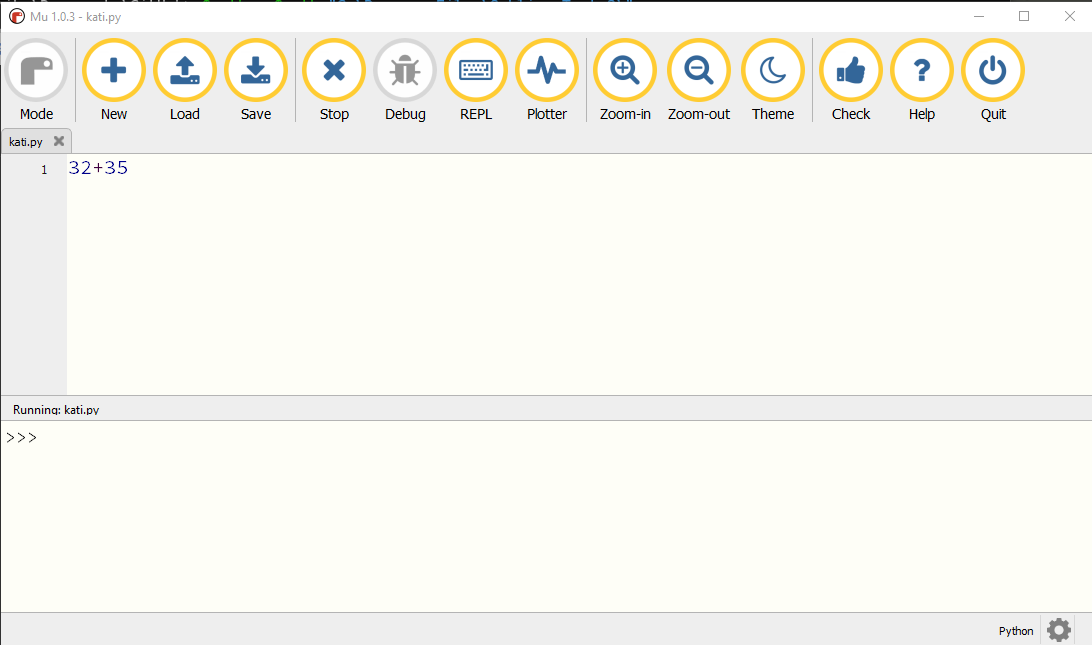
\includegraphics[width=\textwidth]{noprint.png}
\caption{Η εκτέλεση δεν δίνει κάποιο αποτέλεσμα}
\label{noprint}
\end{figure}

Η Python εκτελεί την πράξη $32+35$, και υπολογίζει το αποτέλεσμα. Αν δεν το έκανε και υπήρχε κάποιο πρόβλημα θα εμφάνιζε κάποιο μήνυμα λάθους στο REPL. Το υπολογισμένο αποτέλεσμα δεν εμφανίζεται. Για να εμφανιστεί το αποτέλεσμα πρέπει να χρησιμοποιήσεις την εντολή print (εκτύπωσε). Η εντολή print εκτελείται ως εξής:
\begin{lstlisting}
print(32+35)
\end{lstlisting}
Γράφουμε δηλαδή, print ανοίγουμε παρένθεση, γράφουμε αυτό που θέλουμε να εκτυπωθεί και κλείνουμε την παρένθεση. Όταν εκτελέσουμε το πρόγραμμα με την print τότε εμφανίζεται το αποτέλεσμα στο REPL (εικόνα \ref{withprint}).
\begin{figure}
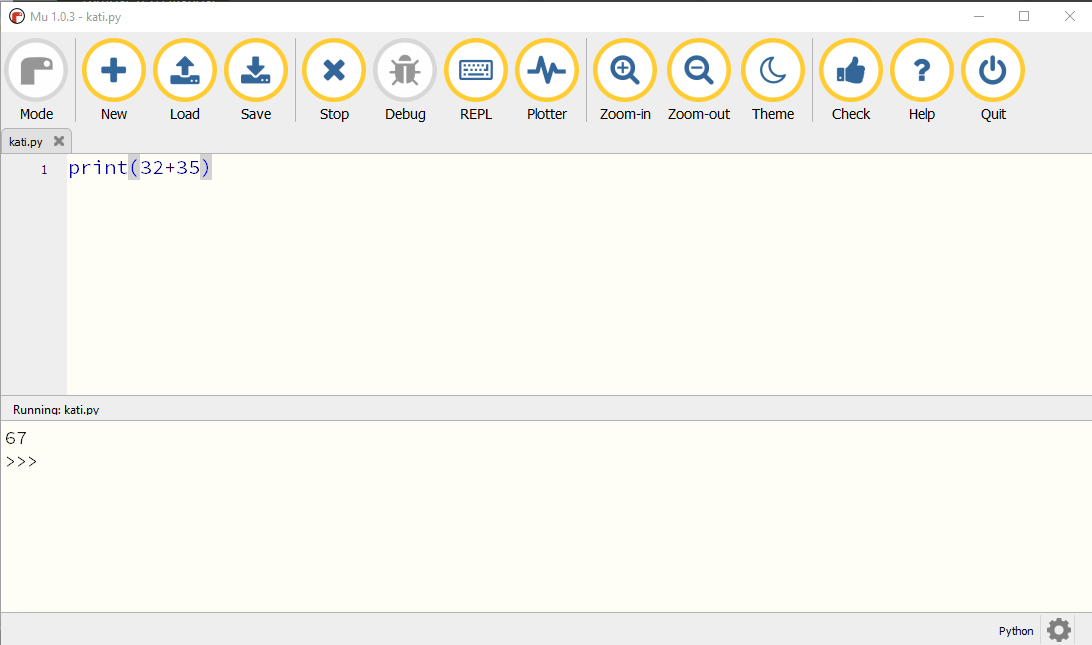
\includegraphics[width=\textwidth]{withprint.png}
\caption{Η εκτέλεση δίνει το αποτέλεσμα της πράξης}
\label{withprint}
\end{figure}
Μόλις έγραψες το πρώτο σου πρόγραμμα στην Python. Μάλιστα το πρόγραμμά σου κάνει κάτι. Υπολογίζει το αποτέλεσμα της πράξης $32+35$.
Μπορείς να αποθηκεύσεις το πρόγραμμά σου στον υπολογιστή σου κάνοντας κλικ στο εικονίδιο Save του Mu (εικόνα \ref{savewithmu}).
\begin{figure}
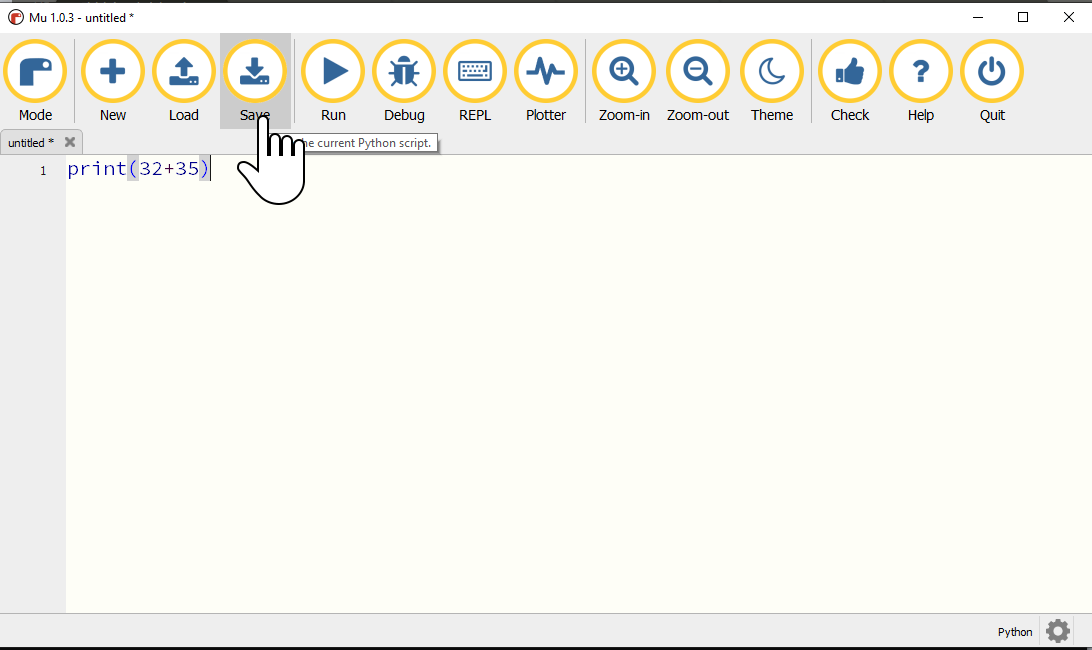
\includegraphics[width=\textwidth]{save.png}
\caption{Αποθήκευση με το Mu}
\label{savewithmu}
\end{figure}

\section{Απαρίθμηση}
Είδαμε ότι η Python μπορεί να κάνει πολύ γρήγορα, πολύπλοκες πράξεις ακόμη και με δυνάμεις, αλλά δεν είδαμε ακόμη τις απλές ασκήσεις που υπάρχουν στις πρώτες σελίδες του βιβλίου. Όπως για παράδειγμα ποιοι είναι οι τρεις προηγούμενοι αριθμοί του 289 και ποιο οι δύο επόμενοι \sel{13}.

Τώρα που μάθαμε να γράφουμε προγράμματα σε Python μπορούμε να αντιμετωπίσουμε αυτό το πρόβλημα με το παρακάτω πρόγραμμα:
\begin{lstlisting}
print(289-3)
print(289-2)
print(289-1)
print(289+1)
print(289+2)
\end{lstlisting}
που δίνει το αποτέλεσμα
\begin{lstlisting}
286
287
288
290
291
\end{lstlisting}

Πιο σωστό θα ήταν να γράψουμε ποιοι αριθμοί είναι οι προηγούμενοι και ποιοι οι επόμενοι. Σε αυτή την περίπτωση θα γράψουμε τις παρακάτω εντολές.
\begin{lstlisting}
print("Οι  προηγούμενοι αριθμοί είναι:")
print(289-3)
print(289-2)
print(289-1)
print("Οι επόμενοι αριθμοί είναι:")
print(289+1)
print(289+2)
\end{lstlisting}

Για να εμφανίσει η print τις λέξεις που θέλουμε πρέπει να τις βάλουμε μέσα σε εισαγωγικά. Η Python υποστηρίζει είτε μονά εισαγωγικά, είτε διπλά. Αυτά εισάγονται συνήθως με το ίδιο κουμπί του πληκτρολογίου (κοντά στο ENTER), είτε με SHIFT ή χωρίς. Θυμήσου να κλείνεις τα εισαγωγικά με τον ίδιο τρόπο που τα άνοιξες. Στο πρόγραμμα Mu τα εισαγωγικά αυτά δεν φαίνονται όπως σε άλλα πρόγραμματα σαν `Εισαγωγικά' ή ``Εισαγωγικά " ή <<Εισαγωγικά>>, αλλά φαίνονται κάπως πιο απλά και ίδια στο άνοιγμα και το κλείσιμο \lstinline{'Εισαγωγικά'} ή  \lstinline{"Εισαγωγικά"}. 

Αν θέλουμε να αλλάξουμε το 289 και να βάλουμε έναν άλλο αριθμό,π.χ. το 132 θα πρέπει να αντικαταστήσουμε το 289 μέσα σε όλες τις εντολές print με το 132.
\begin{lstlisting}
print("Οι προηγούμενοι αριθμοί είναι:")
print(132-3)
print(132-2)
print(132-1)
print("Οι επόμενοι αριθμοί είναι:")
print(132+1)
print(132+2)
\end{lstlisting}

Υπάρχει όμως ένας καλύτερος τρόπος, ο τρόπος αυτός είναι να δώσουμε ένα όνομα στον αριθμό μας. Μπορούμε να πούμε ότι το n είναι το όνομα του αριθμού. Αυτό γίνεται με την εντολή \lstinline{n=132}. Τότε το πρόγραμμά μας γίνεται:
\begin{lstlisting}
n = 132
print("Οι προηγούμενοι αριθμοί είναι:")
print(n-3)
print(n-2)
print(n-1)
print("Οι επόμενοι αριθμοί είναι:")
print(n+1)
print(n+2)
\end{lstlisting}

Μετά την εντολή \lstinline{n=132} η Python ξέρει ότι το n είναι ένα όνομα για το 132 και μπορεί να κάνει πράξεις με αυτό. Για παράδειγμα n+1 κάνει τώρα 133.

Αν θέλουμε να κάνουμε τώρα το ίδιο πρόγραμμα αλλά όχι για το 132 αλλά για το 210, χρειάζεται να αλλάξουμε μόνο μία γραμμή και το πρόγραμμά μας να γίνει ως εξής:
\begin{lstlisting}
n = 210
print("Οι προηγούμενοι αριθμοί είναι:")
print(n-3)
print(n-2)
print(n-1)
print("Οι επόμενοι αριθμοί είναι:")
print(n+1)
print(n+2)
\end{lstlisting}

Στην Python, όταν δίνουμε ένα όνομα σε έναν αριθμό (με τον τελεστή =) τότε δημιουργούμε μια μεταβλητή. Η μεταβλητή έχει ένα όνομα, στην περίπτωσή μας το n, και μια τιμή, στην περίπτωσή μας το 210.

Αν αντί για τους επόμενους δύο αριθμούς θέλαμε τους επόμενους \textbf{δέκα} θα γράφαμε ένα πρόγραμμα όπως το παρακάτω:
\begin{lstlisting}
n = 210
print(n)
print(n+1)
print(n+2)
print(n+3)
print(n+4)
print(n+5)
print(n+6)
print(n+7)
print(n+8)
print(n+9)
print(n+10)
\end{lstlisting}
Το παραπάνω πρόγραμμα εμφανίζει και τον αριθμό μας n, δηλαδή το 210.

Για να μην γράφουμε πολλές εντολές όταν κάνουμε το ίδιο πράγμα χρησιμοποιούμε την εντολή for.
Το πρόγραμμά μας με την for μπορεί να γίνει:
\begin{lstlisting}
n = 210
for i in 0,1,2,3,4,5,6,7,8,9,10:
    print(n+i)
\end{lstlisting}
Όταν γράψεις την for στην Python θα πρέπει να δηλώσεις ποιες εντολές θα εκτελεστούν πολλές φορές. Αυτή η δήλωση γίνεται βάζοντας αυτές τις εντολές λίγο πιο μέσα χρησιμοποιώντας το πλήκτρο κενό ή το πλήκτρο tab. Μια καλή πρακτική είναι να βάζεις τέσσερα κενά. Έτσι, πριν την εντολή \lstinline{print(n+i)} βάζεις τέσσερα κενά δηλαδή \lstinline[showspaces=true]{    print(n+i)}.
Το πρόγραμμα αυτό σημαίνει πως για το i μέσα στο σύνολο 0, 1, 2, 3, \ldots 10 και με αυτή τη σειρά εμφάνισε το n+i. Έτσι το αποτέλεσμα είναι το αναμενόμενο
\begin{lstlisting}
210
211
212
213
214
215
216
217
218
219
220
\end{lstlisting}

Στην Python υπάρχει ένας πιο εύκολος τρόπος να γράψουμε τους αριθμούς από το 0 έως το 10. Αυτός ο τρόπος είναι η εντολή range και συγκεκριμένα η range(11). Η range(11) φτιάχνει τους αριθμούς από το 0 μέχρι το 10 οι οποίοι είναι σε πλήθος 11. 
Έτσι το πρόγραμμά μας γίνεται:
\begin{lstlisting}
n = 210
for i in range(11):
    print(n+i)
\end{lstlisting}

Mπορούμε και να μετρήσουμε τους πρώτους 100 αριθμούς ως εξής:
\begin{lstlisting}
for i in range(100):
    print(i)
\end{lstlisting}

Σκέψου αν θα δεις τον αριθμό 100 στο αποτέλεσμα του παραπάνω προγράμματος.

Μπορούμε να δούμε αριθμούς εύκολα με την Python αλλά θα χρειαστεί ξεχωριστό πρόγραμμα αν θέλουμε να εμφανίζεται το λεκτικό  για κάθε αριθμό.

Ένα τέτοιο πρόγραμμα είναι το παρακάτω:
\begin{lstlisting}
print('μηδέν')
print('ένα')
print('δύο')
print('τρία')
print('τέσσερα')
print('πέντε')
print('έξι')
print('εφτά')
print('οχτώ')
print('εννιά')
print('δέκα')
print('έντεκα')
print('δώδεκα')
print('δεκατρία')
print('δεκατέσσερα')
print('δεκαπέντε')
print('δεκαέξι')
print('δεκαεφτά')
print('δεκαοχτώ')
print('δεκαεννιά')
\end{lstlisting}

Το παραπάνω πρόγραμμα μπορεί να γίνει πιο μαζεμένο με τη χρήση λίστας. Μια λίστα μπορεί να περιέχει τα λεκτικά για κάθε αριθμό. Η λίστα στην Python σημειώνεται με τις τετράγωνες αγκύλες \[ και \]. Τα στοιχεία της χωρίζονται με κόμμα. Έτσι η λίστα που θέλουμε τώρα είναι η εξής:
\begin{lstlisting}
lektika = ['μηδέν','ένα','δύο','τρία','τέσσερα','πέντε','έξι','εφτά','οχτώ','εννιά','δέκα','έντεκα','δώδεκα','δεκατρία','δεκατέσσερα','δεκαπέντε','δεκαέξι','δεκαεφτά','δεκαοχτώ','δεκαεννιά']
\end{lstlisting}
Χρησιμοποιούμε τις τετράγωνες αγκύλες και τον αριθμό του στοιχείου που θέλουμε να προσπελάσουμε σε μια λίστα. Η αρίθμηση της λίστας ξεκινάει από το 0. Έτσι, στη λίστα που βλέπουμε παραπάνω το lektika[0] θα είναι η λέξη 'μηδέν' (θυμηθείτε τα εισαγωγικά), το lektika[1] θα είναι η λέξη 'ένα' κ.ο.κ.

Αν θέλετε μπορείτε να κάνετε μια μικρή δοκιμή στο REPL.
\begin{lstlisting}
>>>lektika = ['μηδέν','ένα','δύο']
>>>lektika[0]
μηδέν
>>>lektika[1]
ένα
>>>lektika[2]
δύο
\end{lstlisting}
Με τη χρήση της λίστας μπορούμε να εμφανίσουμε τους αριθμούς με τη σειρά χρησιμοποιώντας την εντολή for.
\begin{lstlisting}
lektika = ['μηδέν','ένα','δύο','τρία','τέσσερα','πέντε','έξι','εφτά',
'οχτώ','εννιά','δέκα','έντεκα','δώδεκα','δεκατρία',
'δεκατέσσερα','δεκαπέντε','δεκαέξι','δεκαεφτά','δεκαοχτώ',
'δεκαεννιά']
for i in range(20):
    print(lektika[i])
\end{lstlisting}

Όμως παρότι δεν γράφουμε είκοσι φορές την εντολή print πάλι δίνουμε όλα τα ονόματα στο πρόγραμμά μας βάζοντάς τα σε μια λίστα. Μπορούμε να το αποφύγουμε υπολογίζοντας το λεκτικό. Από το δώδεκα και μέτα το λεκτικό ενός αριθμού i είναι το 'δέκα' και μετά το λεκτικό του αριθμού i-10. Για παράδειγμα, το δεκαοχτώ είναι το 'δέκα' ακολουθούμενο από το λεκτικό του αριθμού που προκ΄κυπτει αν αφαιρέσουμε 10 από το 18.
Το πρόγραμμά μας γίνεται:
\begin{lstlisting}
lektika = ['μηδέν','ένα','δύο','τρία','τέσσερα','πέντε','έξι','εφτά',
'οχτώ','εννιά','δέκα','έντεκα','δώδεκα','δεκατρία',
'δεκατέσσερα','δεκαπέντε','δεκαέξι','δεκαεφτά','δεκαοχτώ',
'δεκαεννιά']
for i in range(20):
    if i<=12:
        print(lektika[i])
    else:
        print('δέκα'+lektika[i-10])
\end{lstlisting}

Μάλιστα, το πρόγραμμα υπολογίζει τα λεκτικά από το 13 και μετά και δεν χρειάζεται να τα θυμάται. Μπορούμε να τα διαγράψουμε από τη λίστα.
\begin{lstlisting}
lektika = ['μηδέν','ένα','δύο','τρία','τέσσερα','πέντε','έξι','εφτά',
'οχτώ','εννιά','δέκα','έντεκα','δώδεκα']
for i in range(20):
    if i > 12:
        print('δέκα'+lektika[i-10])
    else:
        print(lektika[i])
\end{lstlisting}

Τώρα μπορούμε να πάμε μέχρι το 29.
\begin{lstlisting}
lektika = ['μηδέν','ένα','δύο','τρία','τέσσερα','πέντε','έξι','εφτά',
'οχτώ','εννιά','δέκα','έντεκα','δώδεκα']
for i in range(30):
    if i>20:
        print('είκοσι' + lektika[i-20])
    elif i > 12:
        print('δέκα'+lektika[i-10])
    else:
        print(lektika[i])
\end{lstlisting}
Το elif είναι συντομογραφία για το else if. Στο σημείο που το έβαλες τώρα σημαίνει αν το i δεν είναι μεγαλύτερο του 20 (else) και είναι μεγαλύτερο από το 12 (if). Άρα το \lstinline{print('δέκα'+lektika[i-10])} γίνεται μόνο αν το i είναι μικρότερο ή ίσο του 20 και μεγαλύτερο από 12.
Το αποτέλεσμα φαίνεται παρακάτω:
\begin{lstlisting}
 ένα  
 δύο 
 τρία 
 τέσσερα 
 πέντε 
 έξι 
 εφτά 
 οχτώ 
 εννιά 
 δέκα 
 έντεκα 
 δώδεκα 
 δέκατρία 
 δέκατέσσερα 
 δέκαπέντε 
 δέκαέξι 
 δέκαεφτά 
 δέκαοχτώ 
 δέκαεννιά 
  (*@\textcolor{blue}{δέκαδέκα}@*) 
 είκοσιένα 
 είκοσιδύο 
 είκοσιτρία 
 είκοσιτέσσερα 
 είκοσιπέντε 
 είκοσιέξι 
 είκοσιεφτά 
 είκοσιοχτώ 
 είκοσιεννιά 
\end{lstlisting}
Οπότε καταλαβαίνουμε ότι το είκοσι χρειάζεται ειδικό χειρισμό. Με τη χρήση της elif μπορούμε να βάλουμε και ειδικό χειρισμό για το 20.
\begin{lstlisting}
lektika = ['μηδέν','ένα','δύο','τρία','τέσσερα','πέντε','έξι','εφτά',
'οχτώ','εννιά','δέκα','έντεκα','δώδεκα']
for i in range(30):
    if i>20:
        print('είκοσι' + lektika[i-20])
    elif i==20:
        print('είκοσι')
    elif i > 12:
        print('δέκα'+lektika[i-10])
    else:
        print(lektika[i])
\end{lstlisting}



\section{Στρογγυλοποίηση}
Το βιβλίο των Μαθηματικών της Α' Γυμνασίου αναφέρει πως
Για να στρογγυλοποιήσουμε έναν φυσικό αριθμό \sel{12}:
\begin{enumerate}
	\item Προσδιορίζουμε την τάξη στην οποία θα γίνει η στρογγυλοποίηση
	\item Εξετάζουμε το ψηφίο της αμέσως μικρότερης τάξης
	\item Αν αυτό το ψηφίο είναι μικρότερο του 5 (δηλαδή 0, 1, 2, 3 ή 4) το ψηφίο αυτό και όλα τα ψηφία των υπόλοιπων τάξεων μηδενίζονται.
	\item Αν είναι μεγαλύτερο ή ίσο του 5 (δηλαδή 5, 6, 7, 8 ή 9) το ψηφίο αυτό και όλα τα ψηφία των υπόλοιπων τάξεων αντικαθίστανται από το 0 και το ψηφίο της τάξης στρογγυλοποίησης αυξάνεται κατά 1.
\end{enumerate}

Ας πούμε ότι θέλουμε να στρογγυλοποιήσουμε τον αριθμό 454.018.512 στα εκατομμύρια. Η απάντηση που περιμένουμε είναι 454 εκατομμύρια.
Για να τα καταφέρουμε θα χρησιμοποιήσουμε την διαίρεση. Όμως στην Python υπάρχουν \emph{δύο} διαιρέσεις μία με το σύμβολο / και μία με το σύμβολο //. Ας δούμε τις διαφορές τους στο REPL.
\begin{lstlisting}
>>> x = 454018512
>>> print(x/1000000)
454.018512
>>> print(x//1000000)
454
\end{lstlisting}
Η <<κανονική>> διαίρεση, με τη μία κάθετο /, δίνει το αποτέλεσμα της διαίρεσης με τα δεκαδικά ψηφία. Η <<ακέραια>> διαίρεση δίνει μόνο τον ακέραιο αριθμό. Δεν μπορούμε να πούμε ότι η ακέραια διαίρεση θα μας δώσει την στρογγυλοποίηση γιατί η ακέραια διαίρεση δεν στρογγυλοποιεί τα δεκαδικά ψηφία αλλά τα απορρίπτει εντελώς. Έτσι, ακόμη και αν είχαμε 454918512 κατοίκους η ακέραια διαίρεση θα δώσει 454 αντί για το στρογγυλοποιημένο που είναι 455.
\begin{lstlisting}
>>> x = 454918512
>>> print(x/1000000)
454.918512
>>> print(x//1000000)
454
\end{lstlisting}

Χρειάζεται επομένως να δούμε το ψηφίο της αμέσως χαμηλότερης τάξης το οποίο είναι το πρώτο δεκαδικό της κανονικής διαίρεσης. Για να το απομονώσουμε αφαιρούμε από το αποτέλεσμα της κανονικής διαίρεσης το ακέραιο μέρος.
\begin{lstlisting}
>>> x = 454018512
>>> x / 1000000 - x // 1000000
0.018511999999986983
\end{lstlisting}
Οπότε τώρα έχουμε δύο ενδεχόμενα αν το αποτέλεσμα αυτής της πράξης είναι μικρότερο από 0.5 όπως παραπάνω τότε το αποτέλεσμα που ψάχνουμε είναι το αποτέλεσμα της ακέραιας διαίρεσης. Αλλιώς πρέπει να προσθέσουμε ένα στο αποτέλεσμα της ακέραιας διαίρεσης.
Αυτό γίνεται με την εντολή if, που σημαίνει στα αγγλικά αν. Για ευκολία μπορούμε να ονομάσουμε d την διαφορά των δύο διαιρέσεων με την εντολή:
\begin{lstlisting}
d = x / 1000000 - x // 1000000
\end{lstlisting}
Επειδή το πρόγραμμα γίνεται μεγαλύτερο τώρα θα το γράψουμε στο πάνω παράθυρο του Mu.
\begin{lstlisting}
x = 454018512
d = x / 1000000 - x // 1000000
if d < 0.5:
    print(x // 1000000)
else:
    print(x // 1000000 + 1)
\end{lstlisting}
Την \lstinline{if} την γράφουμε ως εξής:
\begin{lstlisting}
if συνθήκη:
    εντολές που εκτελούνται
    αν ισχύει η συνθήκη
else:
    εντολές που εκτελούνται
    αν δεν ισχύει η συνθήκη
\end{lstlisting}
Θυμήσου να βάζεις την άνω κάτω τελεία μετά τη συνθήκη και μετά τη λέξη else που σημαίνει αλλιώς.

Αν στο ίδιο πρόγραμμα και βάλεις αντί για 454.018.512 τον αριθμό 454.918.512 θα δεις ότι θα εμφανιστεί το σωστό αποτέλεσμα (455).

Αν θέλεις στρογγυλοποίηση στις χιλιάδες τότε το πρόγραμμά σου γίνεται:
\begin{lstlisting}
x = 454018512
d = x / 1000 - x // 1000
if d < 0.5:
    print(x // 1000)
else:
    print(x // 1000 + 1)
\end{lstlisting}
και το αποτέλεσμα είναι 454019.

\begin{exercise}
Για να γίνει το 454.018.512, 450 εκατομμύρια \sel{12} η στρογγυλοποίηση γίνεται στις δεκάδες των εκατομμυρίων. Μπορείς να γράψεις ένα πρόγραμμα που να στρογγυλοποιεί αριθμούς στις δεκάδες των εκατομμυρίων;
\end{exercise}

\section{Επανάληψη στις πράξεις}
\begin{exercise}
Συμπλήρωσε τον πίνακα τα τετράγωνα και τους κύβους των αριθμών από το 8 μέχρι το 25 \sel{22}.
\end{exercise}
\begin{lstlisting}
for a in range(8,26):
    print(a**2,end =" ")
print()
print()
for a in range(8,26):
    print(a**3,end=" ")
\end{lstlisting}
Το αποτέλεσμα αυτού του προγράμματος είναι:

\begin{lstlisting}
64 81 100 121 144 169 196 225 256 289 324 361 400 441 484 529 576 625 

512 729 1000 1331 1728 2197 2744 3375 4096 4913 5832 6859 8000 9261 
10648 12167 13824 15625
\end{lstlisting}

Η εντολή print μπορεί να πάρει περισσότερα από ένα ορίσματα, το πρώτο όρισμα είναι αυτό που θα εμφανίσει. Το δεύτερο όρισμα που δώσαμε είναι το end και το ορίσαμε ίσο με το κενό (\lstinline{end=" "}) που σημαίνει ότι η print όταν εμφανίσει το πρώτο όρισμα δεν θα αλλάξει γραμμή αλλά θα αφήσει ένα κενό. Η εντολή print() αλλάζει απλά γραμμή.
\begin{exercise}
Βρες τα τετράγωνα των αριθμών 10,20,30,40,50,60,70,80 και 90 \sel{22}.
\end{exercise}
Το πρόγραμμα είναι το εξής:
\begin{lstlisting}
for i in range(10,100,10):
    print(i**2,end=',')
\end{lstlisting}
και το αποτέλεσμα της εκτέλεσης του προγράμματος είναι
\begin{lstlisting}
100,400,900,1600,2500,3600,4900,6400,8100,
\end{lstlisting}

\begin{exercise}
Βρες τους κύβους των αριθμών 10,20,30,40,50
\end{exercise}

\begin{lstlisting}
for i in range(10,60,10):
    print(i**3,end=', ')  
\end{lstlisting}
Το αποτέλεσμα της εκτέλεσης είναι:
\begin{lstlisting}
1000, 8000, 27000, 64000, 125000, 
\end{lstlisting}

\section{Ανάπτυγμα}
\begin{exercise}\sel{21}Να γραφεί το ανάπτυγμα του αριθμόύ 7.604 με χρήση των δυνάμεων του 10.
\end{exercise}
Η απάντηση είναι $7\cdot 10^3 + 6\cdot 10^2 + 0\cdot 10^1 + 4$. 
\chapter{Η έννοια του κλάσματος}
\section{Εισαγωγή}
\begin{exercise}
Ένα βράδυ τρεις φίλοι αγοράζουν μια πίτσα και την χωρίζουν σε οκτώ κομμάτια. Ο ένας έφαγε το ένα, ο δεύτερος τα τρία και ο τρίτος δύο κομμάτια από αυτά που περίσσεψαν.

1. Μπορείς να βρεις το μέρος της πίτσας που έφαγε ο καθένας;

 2. Τι μέρος της πίτσας περίσσεψε;
 \end{exercise}

Ο πρώτος έφαγε το $\frac{1}{8}$ ο δεύτερος τα $\frac{3}{8}$ και ο τρίτος τα $\frac{2}{8}$.
Επομένως και οι τρεις μαζί έφαγαν $1+3+2=6$ κομμάτια, δηλαδή τα $\frac{6}{8}$ της πίτσας. Άρα περίσσεψαν τα υπόλοιπα δύο κομμάτια από τα οκτώ, δηλαδή τα $\frac{2}{8}$ της πίτσας.

Πώς μπορούν να γίνουν πράξεις με κλάσματα στην python; Με τις γνώσεις που ήδη έχουμε εκτελούμε τις παρακάτω εντολές:
\begin{lstlisting}
>>> 1/8
0.125
>>> 3/8
0.375
>>> 2/8
0.25
\end{lstlisting}
Θυμηθείτε ότι η python χρησιμοποιεί την τελεία για τους δεκαδικούς!
Τι μέρος της πίτσας περίσσεψε;
\begin{lstlisting}
>>> 1 - 1/8 - 3/8 - 2/8
0.25
\end{lstlisting}

Όμως, υπάρχει τρόπος η python να υπολογίζει κλάσματα. Απλά θα πρέπει να εισαχθεί το κατάλληλο module. Στην python υπάρχει διαθέσιμο τέτοιο module και ονομάζεται fractions. Για το δεύτερο ερώτημα λοιπόν μπορούμε να κάνουμε το εξής:
\begin{lstlisting}
>>> import fractions
>>> prwtos = fractions.Fraction(1,8)
>>> deuteros = fractions.Fraction(3,8)
>>> tritos = fractions.Fraction(2,8)
>>> 1 - prwtos - deuteros - tritos
Fraction(1, 4)
\end{lstlisting}
Έτσι η python υπολογίζει το αποτέλεσμα με τη μορφή κλάσματος και Fraction(1,4) σημαίνει $\frac{1}{4}$.

Παρατηρείτε ότι γράφουμε το όνομα του module στη συνέχεια την τελεία ``.'' και τέλος το Fraction. Με αυτόν τον τρόπο καλούμε κάτι που υπάρχει μέσα στο module. Υπάρχει όμως και ένας πιο εύκολος τρόπος για να εισάγουμε μόνο τις λειτουργίες που θέλουμε από ένα module και να τις καλούμε.
\begin{lstlisting}
>>> from fractions import Fraction
>>> prwtos = Fraction(1,8)
>>> deuteros = Fraction(3,8)
>>> tritos = Fraction(2,8)
>>> 1 - prwtos - deuteros - tritos
Fraction(1, 4)
\end{lstlisting}
Χρειάζεται προσοχή μόνο αν υπάρχουν περισσότερα από ένα module που πιθανόν να έχουν την ίδια λειτουργία κάτι που δεν ισχύει σε αυτήν την περίπτωση. 

\begin{exercise}
Μια σοκολάτα ζυγίζει 120 gr και έχει 6 ίσα κομμάτια.
(α)   Ποιο μέρος της σοκολάτας είναι το κάθε κομμάτι;
(β)   Πόσα κομμάτια πρέπει να κόψουμε για να πάρουμε 40 gr;
\end{exercise}

Το μέρος της σοκολάτας είναι $\frac{1}{6}$ για να βρούμε πόσα κομμάτια χρειαζόμαστε για 40gr θα πρέπει να βρούμε το βάρος του κομματιού που είναι $\frac{1}{6}\cdot 120$. Τέλος, τα κομμάτια που πρέπει να κόψουμε προκύπτουν από τη διαίρεση των 40 γραμμαρίων με το βάρος του κάθε κομματιού.

\begin{lstlisting}
from fractions import Fraction

sok = Fraction(1,6)
print(sok)
baroskommatiou = sok * 120
kommatia = 40 / baroskommatiou
print('Θα κόψω ' + str(kommatia) + ' κομμάτια!')
\end{lstlisting}
το αποτέλεσμα θα είναι το εξής:
\begin{lstlisting}
1/6
Θα κόψω 2 κομμάτια!
\end{lstlisting}

\begin{exercise}Το καμπαναριό μιας εκκλησίας έχει ύψος 20 m, ενώ η εκκλησία έχει ύψος τα Εικόνα του ύψους του καμπαναριού. Ποιο είναι το ύψος της εκκλησίας;\end{exercise}

\begin{lstlisting}
from fractions import Fraction

>>> kampanario = Fraction(3,5)*20
>>> print(kampanario)
12
\end{lstlisting}
Άρα το ύψος της εκκλησίας είναι 12m.

Στη συνέχεια η εντολή from fractions import Fraction θα υποννοείται ώστε να μην επαναλαμβάνεται συνεχώς. Αν τυχόν την ξεχάσετε το αποτέλεσμα θα έχει το εξής σφάλμα:
\begin{lstlisting}
NameError: name 'Fraction' is not defined
\end{lstlisting}
\begin{exercise} Μια δεξαμενή πετρελαίου σε μια πολυκατοικία, χωράει 2000 lt. Ο διαχειριστής σε μια μέτρηση βρήκε ότι ήταν γεμάτη κατά τα $\frac{3}{4}$. Πόσα λίτρα πετρέλαιο είχε η δεξαμενή;
\end{exercise}
\begin{lstlisting}
>>> dexameni = Fraction(3,4)*2000
>>> print(dexameni)
1500
\end{lstlisting}

Η δεξαμενή έχει 1500 lt.

\begin{exercise}
Tα $\frac{3}{5}$ του κιλού τυρί κοστίζουν 27 €. 

Πόσο κοστίζουν τα $\frac{8}{9}$ του κιλού;
\end{exercise}

\begin{lstlisting}
>>> enaPempto = Fraction(27,3)
>>> tyri = 5*enaPempto
>>> oktwEnata = Fraction(8,9)*tyri
>>> print(oktwEnata)
40
\end{lstlisting}
Τα $\frac{8}{9}$ του τυριού κοστίζουν 40 ευρώ.
\section{Άσκήσεις}
\begin{exercise}
Είναι τα κλάσματα $\frac{3}{4}$, $\frac{2}{3}$, $\frac{7}{9}$, $\frac{10}{9}$, $\frac{18}{20}$ όλα μικρότερα της μονάδας:
\end{exercise}
\begin{lstlisting}
>>> print(Fraction(3,4)<1)
True
>>> print(Fraction(2,3)<1)
True
>>> print(Fraction(7,9)<1)
True
>>> print(Fraction(10,9)<1)
False
>>> print(Fraction(18,20)<1)
True
\end{lstlisting}

\begin{exercise}Τι κλάσμα των μαθητών της τάξης 28 μαθητών είναι οι 4 απόντες;\end{exercise}

\begin{lstlisting}
>>> print(Fraction(4,28))
1/7
\end{lstlisting}

Παρατηρούμε ότι η εντολή Fraction(4,28) κάνει απλοποίηση κλάσματος.

> Αν το $\frac{1}{5}$ ενός κιλού καρύδια είναι 14 καρύδια, το κιλό περιέχει 70 καρύδια;
\begin{lstlisting}
>>> print(14*5 == 70)
\end{lstlisting}
Ναι.

\begin{exercise}
Βρες ποιο μέρος του κιλού είναι τα: (α) 100, (β) 250, (γ) 500, (δ) 600 γραμμάρια.

\end{exercise}

\begin{lstlisting}
>>> print(Fraction(100,1000))
1/10
>>> print(Fraction(250,1000))
1/4
>>> print(Fraction(500,1000))
1/2
>>> print(Fraction(600,1000)).
3/5
\end{lstlisting}

\begin{exercise}
Ποιο μέρος: (α) του μήνα, (β) του εξαμήνου, (γ) του έτους είναι οι 15 ημέρες;
\end{exercise}

\begin{lstlisting}
>>> print(Fraction(15,30))
1/2
>>> print(Fraction(15,180))
1/12
>>> print(Fraction(15,365))
3/73
\end{lstlisting}

\begin{exercise}
Ένα κατάστημα κάνει έκπτωση στα είδη του ίση με τα $\frac{2}{5}$ της αρχικής τιμής τους. Ένα φόρεμα κόστιζε 90 € πριν την έκπτωση. Υπολόγισε πόσα ευρώ έκπτωση έγινε στο φόρεμα και πόσο θα πληρώσουμε για να το αγοράσουμε.
\end{exercise}
\begin{lstlisting}
>>> ekpt = Fraction(2,5)*90
>>> print("Η έκπτωση είναι: " + str(ekpt) + " ευρώ!")
Η έκπτωση είναι: 36 ευρώ!
>>> plir = 90 - ekpt
>>> print("Θα πληρώσουμε: " + str(plir) + " ευρώ!")
Θα πληρώσουμε: 54 ευρώ!
\end{lstlisting}

\begin{exercise}
Σε μία τάξη τα $\frac{3}{8}$ των μαθητών μαθαίνουν αγγλικά. Να βρεις πόσους μαθητές έχει η τάξη, αν γνωρίζεις ότι αυτοί που μαθαίνουν αγγλικά είναι 12 μαθητές.
\end{exercise}

\begin{lstlisting}
>>> print(Fraction(8,3)*12)
32
\end{lstlisting}

\begin{exercise}
Σε ένα ορθογώνιο παραλληλόγραμμο η μια πλευρά του είναι 33 εκατοστά και η άλλη τα $\frac{3}{11}$ της πρώτης. Να βρεις την περίμετρο του ορθογωνίου.
\end{exercise}

\begin{lstlisting}
>>> plevra1 = 33
>>> plevra2 = Fraction(3,11)*plevra1
>>> perimetros = 2*(plevra1 + plevra2)
>>> print(perimetros)
84
\end{lstlisting}

\section{Ισοδύναμα κλάσματα}

\begin{exercise}
Να εξετάσετε αν τα κλάσματα: α) $\frac{3}{5}$ και $\frac{10}{14}$ β) $\frac{3}{8}$ και $\frac{18}{48}$ είναι ισοδύναμα.
\end{exercise}
\begin{lstlisting}
print(Fraction(3,5) == Fraction(10,14))
False
print(Fraction(3,8) == Fraction(18,48))
True
\end{lstlisting}

Έτσι, τα $\frac{3}{5}$ και $\frac{10}{14}$ δεν είναι ισοδύναμα ενώ τα $\frac{3}{8}$ και $\frac{18}{48}$ είναι.

\begin{exercise}Να απλοποιηθεί το κλάσμα $\frac{30}{66}$
\end{exercise}

\begin{lstlisting}
>>> print(Fraction(30,66))
5/11
\end{lstlisting}

\begin{exercise}Να μετατραπούν σε ομώνυμα τα κλάσματα $\frac{3}{5}$, $\frac{2}{3}$ και $\frac{5}{20}$:
\end{exercise}

Επειδή η Fraction κάνει απλοποίηση σε ανάγωγο κλάσμα δεν μπορούμε να επιλέξουμε παρονομαστή, γι' αυτό θα κατασκευάσετε μια συνάρτηση η οποία θα τυπώνει το κλάσμα επιλέγοντας τον παρονομαστή.

\begin{lstlisting}
def tiposemeparonomasti(k,p):
  """
  tiposemeparonomasti(k,p)
  Τύπωσε το κλάσμα k με παρονομαστή p
  """
  if p % k.denominator == 0:#αν το p είναι πολλαπλάσιο
                            #του τρέχοντος παρονομαστή (denominator)
                            #τότε μπορούμε να πολλαπλασιάσουμε
                            #όλο το κλάσμα με έναν συντελεστή
    synt = int(p // k.denominator)
    print(str(k.numerator * synt) + '/' + str(k.denominator * synt))
  else:#αν το p δεν είναι πολλαπλάσιο του τρέχοντος παρονομαστή
       #τότε τυπώνουμε το κλάσμα ως έχει
    print(k)
\end{lstlisting}

Το k.denominator είναι ο παρονομαστής του κλάσματος k.

Αφού φτιάξετε τη συνάρτηση tiposemeparonomasti δοκιμάστε:
\begin{lstlisting}
>>> tiposemeparonomasti(Fraction(3,4),12)
9/12
>>> tiposemeparonomasti(Fraction(1,2),20)
10/20
\end{lstlisting}

Για να κάνουμε ομώνυμα τα κλάσματα βρίσκουμε το Ελάχιστο Κοινό Πολλαπλάσιο (Ε.Κ.Π.) των παρονομαστών. 
Η συνάρτηση για το Ε.Κ.Π. είναι η παρακάτω, αφού το Ε.Κ.Π. δύο αριθμών προκύπτει από το γινόμενο τους αφού το διαιρέσουμε με τον μέγιστο κοινό διαιρέτη (Μ.Κ.Δ. - G.C.D.). Μάλιστα η βιβλιοθήκη fractions περιέχει τη συνάρτηση gcd που υπολογίζει το Μ.Κ.Δ. οπότε:
\begin{lstlisting}
from fractions import gcd
def ekp(a,b):
  return(a*b/gcd(a,b))
\end{lstlisting}

Τέλος συνδυάζοντας τα προηγούμενα το συνολικό πρόγραμμα για να κάνουμε ομώνυμα τα κλάσματα $\frac{3}{5}$, $\frac{2}{3}$ και $\frac{5}{20}$ είναι:

\begin{lstlisting}
from fractions import Fraction,gcd
def tiposemeparonomasti(k,p):
  """
  tiposemeparonomasti(k,p)
  Τύπωσε το κλάσμα k με παρονομαστή p
  """
  if p % k.denominator == 0:#αν το p είναι πολλαπλάσιο
                            #του τρέχοντος παρονομαστή (denominator)
                            #τότε μπορούμε να πολλαπλασιάσουμε
                            #όλο το κλάσμα με έναν συντελεστή
    synt = int(p // k.denominator)
    print(str(k.numerator * synt) + '/' + str(k.denominator * synt))
  else:#αν το p δεν είναι πολλαπλάσιο του τρέχοντος παρονομαστή
       #τότε τυπώνουμε το κλάσμα ως έχει
    print(k)

def ekp(a,b):
  return(a*b/gcd(a,b))    
  
a = Fraction(3,5)
b = Fraction(2,3)
c = Fraction(5,20)
    
koinos = ekp(a.denominator,ekp(b.denominator,c.denominator))
tiposemeparonomasti(a,koinos)
tiposemeparonomasti(b,koinos)
tiposemeparonomasti(c,koinos)
\end{lstlisting}

Μπορούμε να εισάγουμε δύο λειτουργίες από την ίδια βιβλιοθήκη χωρίζοντάς τες με κόμμα ",".
Θυμηθείτε ότι σε ένα κλάσμα a το a.denominator είναι ο παρονομαστής.

Το αποτέλεσμα του προγράμματος είναι:

\begin{lstlisting}
36/60
40/60
15/60
\end{lstlisting}

\begin{exercise}
Να εξετάσετε ποια από τα παρακάτω κλάσματα είναι ισοδύναμα:

(α)$\frac{2}{3},\frac{18}{27}$, 

(β)$\frac{3}{4}$, $\frac{1}{2}$, 

(γ)$\frac{7}{8}$, $\frac{30}{40}$, 

(δ)$\frac{13}{14}$, $\frac{26}{28}$.
\end{exercise}

\begin{lstlisting}
>>> print(Fraction(2,3)==Fraction(18,27))
True
>>> print(Fraction(3,4)==Fraction(1,2))
False
>>> print(Fraction(7,8)==Fraction(30,40))
False
>>> print(Fraction(13,14)==Fraction(26,28))
True
\end{lstlisting}

\begin{exercise}
Να μετατρέψεις καθένα από τα παρακάτω κλάσματα σε ισοδύναμο κλάσμα με παρονομαστή  τον αριθμό 100: 

(α)$\frac{3}{4}$ 

(β)$\frac{8}{5}$ 

(γ)$\frac{4}{20}$ 

(δ)$\frac{5}{2}$ 

(ε)$\frac{60}{75}$

\end{exercise}

Μπορούμε να χρησιμοποιήσουμε την συνάρτηση tiposemeparonomasti
\begin{lstlisting}
>>> tiposemeparonomasti(Fraction(3,4),100)
75/100
>>> tiposemeparonomasti(Fraction(8,5),100)
160/100
>>> tiposemeparonomasti(Fraction(4,20),100)
20/100
>>> tiposemeparonomasti(Fraction(5,2),100)
250/100
>>> tiposemeparonomasti(Fraction(60,75),100)
80/100
\end{lstlisting}

\begin{exercise}Να μετατρέψεις τα παρακάτω κλάσματα σε ισοδύναμα με παρονομαστή τον αριθμό 3:\end{exercise}

\begin{lstlisting}
>>> tiposemeparonomasti(Fraction(10,6),3)
5/3
>>> tiposemeparonomasti(Fraction(50,30),3)
5/3
>>> tiposemeparonomasti(Fraction(18,27),3)
2/3
\end{lstlisting}

\begin{exercise}
Να μετατρέψεις το κλάσμα $\frac{2}{3}$ σε ισοδύναμο κλάσμα με παρονομαστή:(α) 6, και (β) 15.
\end{exercise}

\begin{lstlisting}
>>> tiposemeparonomasti(Fraction(2,3),6)
4/6
>>> tiposemeparonomasti(Fraction(2,3),15)
10/15
\end{lstlisting}

\begin{exercise}
Να απλοποιήσεις τα κλάσματα: (α)$\frac{25}{30}$ (β) $\frac{12}{9}$ (γ) $\frac{32}{56}$
\end{exercise}

\begin{lstlisting}
>>> print(Fraction(25,30))
5/6
>>> print(Fraction(12,9))
4/3
>>> print(Fraction(32,56))
4/7
\end{lstlisting}

\section{Πρόσθεση και αφαίρεση κλασμάτων}

\begin{exercise} Το συνεργείο του Δήμου φύτεψε σε μια μέρα τα $\frac{4}{12}$ μιας πλατείας με λουλούδια. Την επόμενη ήμερα που ο καιρός δεν ήταν καλός φύτεψε μόνο τα $\frac{3}{12}$ της πλατείας. Ποιο τμήμα της πλατείας είχε φυτέψει, συνολικά, στο τέλος της δεύτερης ημέρας;
\end{exercise}

\begin{lstlisting}
>>> print(Fraction(4,12) + Fraction(3,12)(
7/12
\end{lstlisting}

\begin{exercise}Ένα φορτηγό κάλυψε σε μία ώρα τα 2/5 της διαδρομής Πάτρα - Τρίπολη. Ποιο μέρος της διαδρομής του μένει να καλύψει ακόμη;\end{exercise}

\begin{lstlisting}
>>> print(1-Fraction(2,5))
3/5
\end{lstlisting}

\begin{exercise}Μια βρύση γεμίζει, σε 1 ώρα, τα $\frac{2}{5}$ της δεξαμενής. Μια άλλη βρύση γεμίζει το $\frac{1}{3}$ της ίδιας δεξαμενής, επίσης σε 1 ώρα. Αν και οι δύο βρύσες τρέχουν ταυτόχρονα μέσα στη δεξαμενή, τι μέρος της δεξαμενής θα γεμίσουν σε 1 ώρα;
\end{exercise}

\begin{lstlisting}
>>> print(Fraction(2,5)+Fraction(1,3))
11/15
\end{lstlisting}

\begin{exercise}Να υπολογισθεί το άθροισμα 
$$\frac{1}{4}+\frac{2}{4} + 3$$
\end{exercise}

\begin{lstlisting}
>>> print(Fraction(1,4)+Fraction(2,4) + 3)
15/4
\end{lstlisting}

\begin{exercise}Να υπολογισθεί η διαφορά και το άθροισμα των κλασμάτων
$\frac{3}{12}$ και $\frac{7}{20}$.
\end{exercise}

\begin{lstlisting}
>>> print(Fraction(3,12) + Fraction(7,20))
3/5
>>> print(Fraction(7,20) - Fraction(3,12))
1/10
\end{lstlisting}

Για να τυπώσουμε ένα κλάσμα ως μεικτό θα εφαρμόσουμε τα εξής βήματα:
1. Βρίσκουμε το ακέραιο μέρος της διαίρεσης του αριθμητή με τον παρονομαστή έστω $\mu$.
2. Αν το $\mu$ είναι 0 τυπώνουμε το κλάσμα ως έχει (είναι μικρότερο της μονάδας), αλλιώς τυπώνουμε το $\mu$ και στη συνέχεια το κλάσμα που προκύπτει αν από το αρχικό κλάσμα αφαίρεσουμε το $\mu$.

\begin{lstlisting}
def tiposemikto(k):
  m = k.numerator // k. denominator
  if m == 0:
  	print(k)
  else:
  	print(str(m) + " " + str(k-m))
\end{lstlisting}

Για παράδειγμα
\begin{lstlisting}
>>> tiposemikto(Fraction(15,4))
3 3/4
>>> tiposemikto(Fraction(5,2))
2 1/2
>>> tiposemikto(Fraction(38,12))
\end{lstlisting}

\section{Σύγκριση κλασμάτων}

\begin{exercise}
Η Μαρία είπε πως το ροζ χρώμα καταλαμβάνει τα $\frac{9}{48}$, το γαλάζιο τα $\frac{10}{48}$ και το πράσινο τα $\frac{7}{48}$. Ενώ ο Γιάννης είπε ότι το ροζ είναι τα $\frac{3}{16}$, το γαλάζιο τα $\frac{5}{24}$ και το πράσινο το $\frac{1}{8}$ του τετραγώνου.
Ποιος έχει δίκιο και ποιος όχι;
\end{exercise}

\begin{lstlisting}
>>> roz = Fraction(9,48)
>>> print(roz)
3/16
\end{lstlisting}
Άρα και η Μαρία και ο Γιάννης έχουν δίκο όσον αφορά το ροζ χρώμα.

\begin{lstlisting}
>>> galazio = Fraction(10,48)
>>> print(galazio)
5/24
\end{lstlisting}
Άρα και η Μαρία και ο Γιάννης έχουν δίκο όσον αφορά το γαλάζιο χρώμα.

Τέλος, όσον αφορά το πράσινο προκύπτει ότι:
\begin{lstlisting}
>>> prasino = Fraction(7,48)
>>> print(prasino)
7/48
>>> Fraction(7,48) == Fraction(1,8)
False
>>> Fraction(7,48) > Fraction(1,8)
True
\end{lstlisting}
Δηλαδή, το $\frac{7}{48}$ είναι μεγαλύτερο από το $\frac{1}{8}$.
%Σχήμα

\subsection{Παραδείγματα}

\begin{exercise}Να συγκριθούν τα κλάσματα $\frac{7}{10}$ και $\frac{7}{15}$\end{exercise}

\begin{lstlisting}
>>> Fraction(7,10) > Fraction(7,15)
True
\end{lstlisting}

Άρα, $\frac{7}{10}>\frac{7}{15}$.

\begin{exercise}Να συγκριθούν τα κλάσματα: $\frac{5}{8}$ και $\frac{4}{9}$.\end{exercise}

\begin{lstlisting}
>>> Fraction(5,8) > Fraction(4,9)
True
\end{lstlisting}

Δεν χρειάζεται να τα μετατρέψουμε σε ομώνυμα, η python λύνει το πρόβλημα της σύγκρισης με τον δικό της τρόπο.

\begin{exercise}
Σύγκρινε τα κλάσματα (α) $\frac{3}{7}$ και $\frac{5}{7}$, (β) $\frac{3}{5}$ και $\frac{3}{9}$ και (γ) $\frac{4}{5}$ και $\frac{8}{12}$.
\end{exercise}

\begin{lstlisting}
>>> Fraction(3,7) < Fraction(5,7)
True
>>> Fraction(3,5) > Fraction(3,9)
True
>>> Fraction(4,5) > Fraction(8,12)
True
\end{lstlisting}

\begin{exercise}Βάλε σε σειρά τα κλάσματα $\frac{3}{5}$, $\frac{8}{15}$, $\frac{5}{10}$, $\frac{20}{15}$, $\frac{7}{5}$\end{exercise}

\begin{lstlisting}
>>> lista = [Fraction(31,10),Fraction(8,15),Fraction(5,10),
Fraction(20,15),Fraction(7,5)]
>>> print(",".join([str(x) for x in sorted(lista)]))
1/2,8/15,4/3,7/5,31/10
\end{lstlisting}

\section{Πολλαπλασιασμός κλασμάτων}

\begin{exercise}Να βρεθεί το γινόμενο $\frac{3}{7}\cdot\frac{70}{6}\cdot\frac{8}{5}$\end{exercise}

\begin{lstlisting}
>>> Fraction(3,7)*Fraction(70,6)*Fraction(8,5)
8
\end{lstlisting}

\begin{exercise}Σε ένα σχολείο με 252 μαθητές τα $\frac{5}{9}$ είναι αγόρια. Πόσα είναι τα αγόρια και πόσα είναι τα κορίτσια;
\end{exercise}

\begin{lstlisting}    
>>> agoria,koritsia = 252*Fraction(5,9),252-252*Fraction(5,9)
>>> print(agoria)
140
>>> print(koritsia)
112
\end{lstlisting}

\begin{exercise}Υπολόγισε τα γινόμενα $3\cdot\frac{3}{4}$, $7\cdot\frac{10}{14}$, $\frac{4}{2}\cdot 2$, $\frac{5}{100}\cdot 10$\end{exercise}

\begin{lstlisting}
>>> x = 3*Fraction(3,4)
>>> print(x)
9/4
>>> x = 7*Fraction(10,14)
>>> print(x)
5
>>> x = Fraction(4,2)*2
>>> print(x)
4
>>> x = Fraction(5,100)*10
>>> print(x)
1/2
\end{lstlisting}

\begin{exercise}
Βρες τα γινόμενα $\frac{2}{5}\cdot\frac{7}{8}$, $\frac{8}{10}\cdot\frac{100}{5}$, $\frac{4}{9}\cdot\frac{5}{9}$, $\frac{3}{2}\cdot\frac{2}{15}$
\end{exercise}

\begin{lstlisting}
>>> x = Fraction(2,5)*Fraction(7,8)
>>> print(x)
7/20
>>> x = Fraction(8,10)*Fraction(100,5)
>>> print(x)
16
>>> x = Fraction(4,9)*Fraction(5,9)
>>> print(x)
20/81
>>> x = Fraction(3,2)*Fraction(2,15)
>>> print(x)
1/5
\end{lstlisting}

\begin{exercise}
Συμπλήρωσε τον πίνακα:
\end{exercise}

\begin{table}
\begin{tabular}{|c|c|c|c|c|}
                                      & $\frac{5}{7}$& $\frac{3}{2}$& $1$& $\frac{3}{4}$\\\hline
$\frac{7}{5}$              &                         &                         &       &                         \\\hline
$\frac{2}{3}$              &                         &                         &       &                         \\\hline
$1$                                &                         &                         &       &                         \\\hline
$\frac{4}{3}$              &                         &                         &       &                         \\\hline
\end{tabular}
\end{table}

Ο πίνακας αυτός μπορεί να εμφανιστεί με το παρακάτω πρόγραμμα:

\begin{lstlisting}
from fractions import Fraction

ori = [Fraction(5,7),Fraction(3,2),1,Fraction(3,4)]
kat = [Fraction(7,5),Fraction(2,3),1,Fraction(4,3)]
print(" "*5+", ",end=" ")
for orizontio in ori:
    print(str(orizontio).rjust(5),end=", ")
print()
print("-"*35)
for katheto in kat:
    print(str(katheto).rjust(5),end=", |")
    for orizontio in ori:
        print(str(orizontio*katheto).rjust(5),end=", ")
    print()
\end{lstlisting}
και το αποτέλεσμα του προγράμματος είναι:
\begin{table}
\begin{tabular}{|c|c|c|c|c|}
                        & $\frac{5}{7}$   & $\frac{3}{2}$    & $1$                & $\frac{3}{4}$\\\hline
$\frac{7}{5}$&    $1$                   &$\frac{21}{10}$&$\frac{7}{5}$&$\frac{21}{20}$\\\hline
$\frac{2}{3}$&$\frac{10}{21}$ & $1$                      & $\frac{2}{3}$&  $\frac{1}{2}$      \\\hline
$1$                  &$\frac{5}{7}$     & $\frac{3}{2}$    &     $1$               &   $\frac{3}{4}$      \\\hline
$\frac{4}{3}$&  $ \frac{20}{21}$& $2$                   &      $\frac{4}{3}$ &  $1$ \\\hline
\end{tabular}
\end{table}

\begin{exercise}
Υπολόγισε τα γινόμενα $2\frac{1}{3}\cdot\frac{3}{21}$, $4\frac{1}{5}\cdot 2\frac{1}{2}$, $3\frac{1}{8}\cdot 10$, $1\frac{2}{3}\cdot\frac{3}{2}$
\end{exercise}
\begin{lstlisting}
x = (2+Fraction(1,3))*Fraction(3,21)
print(x)

x = (4+Fraction(1,5))*(2+Fraction(1,2))
print(x)

x = (3+Fraction(1,8))*10
print(x)

x = (1+Fraction(2,3))*Fraction(3,2)
print(x)
\end{lstlisting}
και το αποτέλεσμα είναι
\begin{lstlisting}
1/3
21/2
125/4
5/2
\end{lstlisting}
\begin{exercise}
Να βρεις τους αντίστροφους των αριθμών $\frac{4}{7}$, $72$, $\frac{5}{8}$, $\frac{1}{3}$, $\frac{739}{8}$, $1$
\end{exercise}
\begin{lstlisting}
print(1/Fraction(4,7))
print(1/Fraction(72))
print(1/Fraction(5,8))
print(1/Fraction(1,3))
print(1/Fraction(739,8))
print(1/Fraction(1))
\end{lstlisting}
και το αποτέλεσμα είναι:
\begin{lstlisting}
7/4
1/72
8/53
8/739
1
\end{lstlisting}
\begin{exercise}
Ο Κώστας ήπιε τα $\frac{2}{3}$ από ένα μπουκάλι, που περιείχε αναψυκτικό όγκου $1\frac{1}{2}$ του λίτρου. Πόσα λίτρα αναψυκτικού ήπιε;
\end{exercise}
\begin{lstlisting}
print(Fraction(2,3)*(1+Fraction(1,2)))
\end{lstlisting}
που δίνει αποτέλεσμα
\begin{lstlisting}
1
\end{lstlisting}
Ο Κώστας ήπιε $1$ λίτρο αναψυκτικού.

\begin{exercise}
Υπολόγισε τα εξαγόμενα των πράξεων $\frac{6}{5} + \frac{3}{5}\cdot\frac{1}{4}$, $(\frac{6}{5} + \frac{3}{5})\cdot\frac{1}{4}$,
$\frac{6}{5} - \frac{3}{5}\cdot\frac{1}{4}$
\end{exercise}

\begin{lstlisting}
x = Fraction(6,5) + Fraction(3,5)*Fraction(1,4)
print(x)

x = (Fraction(6,5)+Fraction(3,5))*Fraction(1,4)
print(x)

x = (Fraction(6,5)-Fraction(3,5))*Fraction(1,4)
print(x)
\end{lstlisting}
Το αποτέλεσμα είναι το εξής:
\begin{lstlisting}
27/20
9/20
3/20
\end{lstlisting}
\begin{exercise}
Όμοια $(\frac{7}{3}+\frac{2}{15})\cdot \frac{3}{8}$, $(\frac{7}{3}+\frac{2}{15})\cdot \frac{3}{8}$, $\frac{7}{3}-\frac{2}{15}\cdot \frac{3}{8}$
\end{exercise}
\begin{lstlisting}
x = (Fraction(7,3)+Fraction(2,15))*Fraction(3,8)
print(x)

x = (Fraction(7,3)-Fraction(2,15))*Fraction(3,8)
print(x)

x = Fraction(7,3)-Fraction(2,15)*Fraction(3,8)
print(x)
\end{lstlisting}
και το αποτέλεσμα είναι:
\begin{lstlisting}
37/40
33/40
137/60
\end{lstlisting}


%x = Fraction(Fraction(2,3),Fraction(10,9))
%print(x)
%
%x = Fraction(4,Fraction(9,8))
%print(x)
%
%x = Fraction(Fraction(7,10),5)
%print(x)
%
%x = Fraction((Fraction(3,10)+Fraction(1,2)),(Fraction(4,3)-Fraction(4,6)))
%print(x)
%
%def rhind(x):
%  """calculate (2/3)*(1/x)"""
%  if not x%2 == 1:
%    return(None)
%  else:
%    return(Fraction(1,2*x)+Fraction(1,6*x))
 %
%print(rhind(7) == Fraction(2,3)*Fraction(1,7))
%\end{lstlisting}

\end{document}